% Options for packages loaded elsewhere
\PassOptionsToPackage{unicode}{hyperref}
\PassOptionsToPackage{hyphens}{url}
\PassOptionsToPackage{dvipsnames,svgnames,x11names}{xcolor}
%
\documentclass[
  10pt,
]{article}
\usepackage{amsmath,amssymb}
\usepackage{iftex}
\ifPDFTeX
  \usepackage[T1]{fontenc}
  \usepackage[utf8]{inputenc}
  \usepackage{textcomp} % provide euro and other symbols
\else % if luatex or xetex
  \usepackage{unicode-math} % this also loads fontspec
  \defaultfontfeatures{Scale=MatchLowercase}
  \defaultfontfeatures[\rmfamily]{Ligatures=TeX,Scale=1}
\fi
\usepackage{lmodern}
\ifPDFTeX\else
  % xetex/luatex font selection
\fi
% Use upquote if available, for straight quotes in verbatim environments
\IfFileExists{upquote.sty}{\usepackage{upquote}}{}
\IfFileExists{microtype.sty}{% use microtype if available
  \usepackage[]{microtype}
  \UseMicrotypeSet[protrusion]{basicmath} % disable protrusion for tt fonts
}{}
\makeatletter
\@ifundefined{KOMAClassName}{% if non-KOMA class
  \IfFileExists{parskip.sty}{%
    \usepackage{parskip}
  }{% else
    \setlength{\parindent}{0pt}
    \setlength{\parskip}{6pt plus 2pt minus 1pt}}
}{% if KOMA class
  \KOMAoptions{parskip=half}}
\makeatother
\usepackage{xcolor}
\usepackage[margin=22mm]{geometry}
\usepackage{longtable,booktabs,array}
\usepackage{calc} % for calculating minipage widths
% Correct order of tables after \paragraph or \subparagraph
\usepackage{etoolbox}
\makeatletter
\patchcmd\longtable{\par}{\if@noskipsec\mbox{}\fi\par}{}{}
\makeatother
% Allow footnotes in longtable head/foot
\IfFileExists{footnotehyper.sty}{\usepackage{footnotehyper}}{\usepackage{footnote}}
\makesavenoteenv{longtable}
\usepackage{graphicx}
\makeatletter
\def\maxwidth{\ifdim\Gin@nat@width>\linewidth\linewidth\else\Gin@nat@width\fi}
\def\maxheight{\ifdim\Gin@nat@height>\textheight\textheight\else\Gin@nat@height\fi}
\makeatother
% Scale images if necessary, so that they will not overflow the page
% margins by default, and it is still possible to overwrite the defaults
% using explicit options in \includegraphics[width, height, ...]{}
\setkeys{Gin}{width=\maxwidth,height=\maxheight,keepaspectratio}
% Set default figure placement to htbp
\makeatletter
\def\fps@figure{htbp}
\makeatother
\setlength{\emergencystretch}{3em} % prevent overfull lines
\providecommand{\tightlist}{%
  \setlength{\itemsep}{0pt}\setlength{\parskip}{0pt}}
\setcounter{secnumdepth}{-\maxdimen} % remove section numbering
% definitions for citeproc citations
\NewDocumentCommand\citeproctext{}{}
\NewDocumentCommand\citeproc{mm}{%
  \begingroup\def\citeproctext{#2}\cite{#1}\endgroup}
\makeatletter
 % allow citations to break across lines
 \let\@cite@ofmt\@firstofone
 % avoid brackets around text for \cite:
 \def\@biblabel#1{}
 \def\@cite#1#2{{#1\if@tempswa , #2\fi}}
\makeatother
\newlength{\cslhangindent}
\setlength{\cslhangindent}{1.5em}
\newlength{\csllabelwidth}
\setlength{\csllabelwidth}{3em}
\newenvironment{CSLReferences}[2] % #1 hanging-indent, #2 entry-spacing
 {\begin{list}{}{%
  \setlength{\itemindent}{0pt}
  \setlength{\leftmargin}{0pt}
  \setlength{\parsep}{0pt}
  % turn on hanging indent if param 1 is 1
  \ifodd #1
   \setlength{\leftmargin}{\cslhangindent}
   \setlength{\itemindent}{-1\cslhangindent}
  \fi
  % set entry spacing
  \setlength{\itemsep}{#2\baselineskip}}}
 {\end{list}}
\usepackage{calc}
\newcommand{\CSLBlock}[1]{\hfill\break\parbox[t]{\linewidth}{\strut\ignorespaces#1\strut}}
\newcommand{\CSLLeftMargin}[1]{\parbox[t]{\csllabelwidth}{\strut#1\strut}}
\newcommand{\CSLRightInline}[1]{\parbox[t]{\linewidth - \csllabelwidth}{\strut#1\strut}}
\newcommand{\CSLIndent}[1]{\hspace{\cslhangindent}#1}
\ifLuaTeX
\usepackage[bidi=basic]{babel}
\else
\usepackage[bidi=default]{babel}
\fi
\babelprovide[main,import]{english}
% get rid of language-specific shorthands (see #6817):
\let\LanguageShortHands\languageshorthands
\def\languageshorthands#1{}
% Keep long identifiers and wide descriptive tables legible in the draft.
\emergencystretch=3em
\setlength{\tabcolsep}{3pt}
\usepackage{etoolbox}
\BeforeBeginEnvironment{longtable}{\begingroup\footnotesize}
\AfterEndEnvironment{longtable}{\endgroup}
\usepackage{float}
\floatplacement{figure}{H}
\ifLuaTeX
  \usepackage{selnolig}  % disable illegal ligatures
\fi
\usepackage{bookmark}
\IfFileExists{xurl.sty}{\usepackage{xurl}}{} % add URL line breaks if available
\urlstyle{same}
\hypersetup{
  pdftitle={Observable-Dependent Interference Detection: Measured GNSS Evidence and Payload-Aware GEO Simulation},
  pdfauthor={Anonymous research draft --- author list pending},
  pdflang={en},
  colorlinks=true,
  linkcolor={Maroon},
  filecolor={Maroon},
  citecolor={Blue},
  urlcolor={Blue},
  pdfcreator={LaTeX via pandoc}}

\title{Observable-Dependent Interference Detection: Measured GNSS
Evidence and Payload-Aware GEO Simulation}
\author{Anonymous research draft --- author list pending}
\date{26 October 2026 --- Manuscript V1}

\begin{document}
\maketitle
\begin{abstract}
Interference-detection results depend on what an observation represents,
which recordings are available, and how an operating threshold is
calibrated. We report a reproducibility and comparative-methods study
with three explicitly separate evidence streams: measured GNSS receiver
telemetry and rendered spectrograms, measured solid-state amplifier
input/output data, and controlled GEO reference-channel simulations.
Three fixed CPU scores---native level, clean diagonal distance, and
binary centroid margin---are evaluated without test-driven score
reversal or method selection. Their LC AUROCs are 0.9842, 0.9677, and
0.9142; their FIOT AUROCs are 0.2590, 0.8578, and 0.5946. LC performance
is conditional on 120 nonempty records out of 159 published test
records; missing recordings cannot silently become correct negatives.
Thresholds calibrated on 38 and 69 clean training-partition records
target a nominal 5\% false-alarm probability but do not establish
population-level precision. Existing measured-amplifier fits and
simulated carrier-observability diagnostics supply complementary support
and limitations, not a common generalization benchmark. We retain
negative findings, uncertain session independence, unresolved license
statements, and inaccessible satellite comparisons. The contribution is
an auditable evaluation of release, representation, coverage, and
calibration limits, not a new classifier, measured GEO validation, or
confirmed advantage of payload-aware open-set recognition.
\end{abstract}

\section{Introduction}\label{introduction}

Satellite interference monitoring is an inference problem constrained by
its observation point. A receiver may expose channel-quality telemetry,
a rendered image, calibrated spectra, or complex samples. These are
different experimental objects. A detector that responds to changes in a
receiver's reported strength need not operate on an image whose colors
were produced by an undocumented rendering pipeline. Likewise, an uplink
interferer passing through a satellite amplifier is physically different
from a downlink mixture added after that amplifier. Treating all such
data as interchangeable can make a benchmark look more operationally
meaningful than its evidence permits.

Prior satellite studies already investigate on-board detection and
cancellation, neural interference detection, and prediction of received
spectra (Politis et al. 2017; Henarejos, Vázquez, and Pérez-Neira 2019;
Pellaco, Singh, and Jaldén 2019). Public SmartSpace tasks address
on-board interference locations and NGSO-to-GSO interference detection
(Daoud et al. 2023; Saifaldawla et al. 2024). Measured GNSS studies
already combine multiple modalities and examine model reliability and
data discrepancies (Brieger et al. 2022; Heublein et al. 2024).
Consequently, neither the use of elementary detection scores nor the
observation that data representations matter is a new algorithmic
contribution.

Our narrower question is operationally concrete: \textbf{what can
actually be reproduced from the released files, with publisher splits
preserved and a threshold chosen without inspecting test performance,
and which satellite claims remain unsupported?} We examine the
consequences of empty receiver records, repeated image crops,
uncalibrated RGB values, limited calibration populations, and
distinctions between hardware measurements and reference-channel
simulation. These issues are easy to lose when results are reduced to a
single accuracy number.

The study makes three bounded contributions. First, it documents and
checks the actual released LC/FIOT representations, recording-level
splits, availability coverage, and native labels. Second, it presents
all three frozen detection scores and clean-calibrated operating points,
retaining a strongly negative image-level result and explicit
conditional uncertainty. Third, it connects those empirical limits to
separately identified measured-amplifier support and GEO observability
diagnostics. This connection is an interpretation across evidence types,
\textbf{not an executed cross-domain transfer experiment}.

The original project proposed a reference-traceable generator (C1), a
plan-conditioned dual-polarization open-set recognizer (C2), and a
quantified payload gap (C3). Here C1 contributes limited simulation
methodology; confirmatory C2 and C3 claims are not made. This manuscript
is positioned as a reproducibility/comparative-methods paper. Its
suitability for a particular venue depends on whether that venue values
the release-level audit and calibrated negative evidence; combining
existing baseline results alone would not support a claim of a new
recognition method.

\section{Related work and scope of
comparison}\label{related-work-and-scope-of-comparison}

\subsection{Satellite interference
observations}\label{satellite-interference-observations}

Politis and colleagues study weak satellite interference detection after
signal cancellation (Politis et al. 2017). Such work motivates
residual-domain detection but does not make every cancellation residual
equivalent: observation point, receiver knowledge, reconstruction
errors, and payload distortion matter. Henarejos and colleagues
investigate deep-learning interference detection and classification
(Henarejos, Vázquez, and Pérez-Neira 2019), while Pellaco and colleagues
predict spectra for satellite interference detection (Pellaco, Singh,
and Jaldén 2019). These studies establish prior satellite-learning
approaches; we do not claim to introduce satellite anomaly detection.

The SmartSpace on-board release provides clean and interfered
subband-location labels; the NGSO release supplies clean
training/validation data and a mixed test population (Daoud et al. 2023;
Saifaldawla et al. 2024; University of Luxembourg SmartSpace n.d.).
Their tasks differ from an eight-type GEO open-set benchmark. The
available source descriptions do not justify assuming operator carrier
plans, paired polarization observations, calibrated absolute RF power,
or measured GEO field data. We provide no numerical comparison with
their reported methods because the official raw downloads were
inaccessible to this study.

\subsection{Measured GNSS and amplifier
evidence}\label{measured-gnss-and-amplifier-evidence}

Brieger and colleagues introduce multimodal GNSS interference
classification and reliability analysis; the LC/FIOT source release
cites that work (Brieger et al. 2022, 2026). Heublein and colleagues
examine supervised/unsupervised robustness and real-world data
discrepancies (Heublein et al. 2025, 2024). Their analysis is direct
prior work, not evidence that our elementary scores are novel. Our
distinct emphasis is the exact released-file representation, coverage,
crop-parent separation and clean-threshold behavior of a reproducible
bounded comparison. We do not reproduce their full model suite or claim
a method-level improvement over it.

OpenDPD supplies measured power-amplifier data and modeling tools (Wu et
al. 2024). We reuse an existing train-fitted, validation-selected
memory-polynomial artifact, rather than repeating its estimation. The
devices are solid-state Doherty amplifiers, not satellite traveling-wave
tube amplifiers (TWTAs). ETSI reference transponder descriptions and
digitized reference responses serve a different role in the GEO
simulation (ETSI 2014, 2021). Saleh's model is a documented analytical
alternative (Saleh 1981); it is not substituted for the project's
default digitized reference response.

\subsection{What is and is not
compared}\label{what-is-and-is-not-compared}

The measured GNSS experiments compare three scores \textbf{within each
source}. LC and FIOT models are fitted separately. Measured PA fits
assess reproduction of amplifier outputs; their NMSE is not a detection
metric. GEO diagnostics assess controlled physical contrasts; they are
not field measurements or learned recognition benchmarks. We neither
pool these populations nor rank the three evidence streams on a shared
accuracy scale. The prior literature verification record in
\texttt{paper/literature\_audit.md} distinguishes primary full-text
checks, publisher metadata, dataset descriptions, and inaccessible
source documents.

\section{Data, labels, access, and legal
constraints}\label{data-labels-access-and-legal-constraints}

\subsection{Measured GNSS receiver telemetry and
images}\label{measured-gnss-receiver-telemetry-and-images}

The Fraunhofer laboratory release is pinned to the author-repository
snapshot identified in the cited release and evidence supplement
(Brieger et al. 2026). The actual binary archives, rather than Git LFS
pointer files, were obtained. LC contains 744 NPY files, of which 736
appear in the published label lists. Eight unlabelled files are excluded
without imputation of class labels. Nonempty LC arrays have 308 columns
and nine or ten rows; 184 labelled arrays have zero rows. No inference
is made about why a recording is empty.

FIOT files are \(512\times243\times3\) integer RGB spectrogram images.
The three channels are colors, not polarizations. They are neither raw
IQ nor calibrated power spectral densities. The publisher's 5,268/1,458
train/test crop split corresponds to 878/243 parent IDs with six crops
per parent. We retain only crop index zero for every parent. This
prevents treating repeated views as independent samples and bounds
processing; it does not demonstrate independent acquisition sessions.

\textbf{Table T1a. Measured GNSS populations. Counts are recording
parents after crop selection.}

\begin{longtable}[]{@{}
  >{\raggedright\arraybackslash}p{(\columnwidth - 8\tabcolsep) * \real{0.1579}}
  >{\raggedleft\arraybackslash}p{(\columnwidth - 8\tabcolsep) * \real{0.2105}}
  >{\raggedleft\arraybackslash}p{(\columnwidth - 8\tabcolsep) * \real{0.2105}}
  >{\raggedleft\arraybackslash}p{(\columnwidth - 8\tabcolsep) * \real{0.2105}}
  >{\raggedleft\arraybackslash}p{(\columnwidth - 8\tabcolsep) * \real{0.2105}}@{}}
\toprule\noalign{}
\begin{minipage}[b]{\linewidth}\raggedright
Source
\end{minipage} & \begin{minipage}[b]{\linewidth}\raggedleft
Published train/test
\end{minipage} & \begin{minipage}[b]{\linewidth}\raggedleft
Usable train/test
\end{minipage} & \begin{minipage}[b]{\linewidth}\raggedleft
Empty train/test
\end{minipage} & \begin{minipage}[b]{\linewidth}\raggedleft
Test clean/positive
\end{minipage} \\
\midrule\noalign{}
\endhead
\bottomrule\noalign{}
\endlastfoot
LC receiver features & 577 / 159 & 432 / 120 & 145 / 39 & 44 / 76
usable \\
FIOT RGB, crop 0 & 878 / 243 & 878 / 243 & 0 / 0 & 81 / 162 \\
\end{longtable}

LC's full labelled test set contains 59 clean and 100 positive records.
Its empty test records comprise 15 clean and 24 positive cases. Empty
records are \textbf{abstentions}, not correct clean predictions. Thus LC
usable test coverage is \(120/159=75.5\%\). Native labels are retained:
0=None/clean, 1=Noise, 2=Chirp, 3=FreqHopper, 4=Modulated, 5=Multitone,
6=Pulsed, 7=Cw, and 8=Tone. The released LC population has no class-7
support; both usable test sets have only two Tone records. The labels
are not remapped to the GEO taxonomy.

No parent ID or nonempty file hash overlaps the retained train/test
partitions. This catches crop repetition and exact duplicate bytes, not
all physical dependencies. Acquisition day, session and jammer-setup
independence cannot be established from the supplied identifiers. In
particular, we do not describe this split as an unseen-site,
unseen-session or unseen-emitter evaluation.

\subsection{Satellite comparison data and amplifier
measurements}\label{satellite-comparison-data-and-amplifier-measurements}

\textbf{Table T1b. Additional sources and observation boundaries. Counts
here are not pooled with T1a.}

\begin{longtable}[]{@{}
  >{\raggedright\arraybackslash}p{(\columnwidth - 4\tabcolsep) * \real{0.3333}}
  >{\raggedright\arraybackslash}p{(\columnwidth - 4\tabcolsep) * \real{0.3333}}
  >{\raggedright\arraybackslash}p{(\columnwidth - 4\tabcolsep) * \real{0.3333}}@{}}
\toprule\noalign{}
\begin{minipage}[b]{\linewidth}\raggedright
Source
\end{minipage} & \begin{minipage}[b]{\linewidth}\raggedright
Published representation/split
\end{minipage} & \begin{minipage}[b]{\linewidth}\raggedright
Actual use and boundary
\end{minipage} \\
\midrule\noalign{}
\endhead
\bottomrule\noalign{}
\endlastfoot
SmartSpace on-board & Full/reduced FFT magnitude or complex data; 12,000
train and 3,000 validation; clean plus five subband locations & Zero raw
files obtained; no separate test described; no measured result here \\
SmartSpace NGSO & 800 magnitude values; 11,500 clean train, 1,302 clean
validation, 4,470 mixed test & Zero raw files obtained; numeric
test-positive convention unverified; no result here \\
OpenDPD APA/DPA & Measured paired input/output IQ, native
train/validation/test files & Existing PA fit artifact reused; no new
fitting or measurement \\
GEO reference simulation & Controlled multicarrier observations and
separately versioned pilots & Existing committed summaries only; no new
generation or protected observations read \\
\end{longtable}

On 26 October 2026 the two official SmartSpace download links redirected
to Microsoft sign-in HTML. An HTTP200 login response is not an acquired
dataset. A functioning research share or owner-granted folder
read/download permission is needed. Whether external Entra guests,
particular institutional accounts, MFA or expiry rules apply remains an
owner-side question. An access-request draft exists; it was not sent as
part of this manuscript task. Neither MAT keys nor paired-view/group
identities can be verified without the files. Appended INR, off-axis
parameters and labels would not be legitimate detector features.

The LC/FIOT Zenodo API license field states CC BY-SA 4.0, whereas the
source README/description states CC BY-NC-SA 4.0. This discrepancy is
unresolved and must be clarified for the intended publication. Local
research followed the more restrictive noncommercial statement; this is
not a legal resolution. SmartSpace states research-only use. OpenDPD
repository code carries Apache-2.0, but the inspected data descriptions
do not separately settle all measurement-data rights. We redistribute no
third-party raw archives, NPY files or CSVs. All plotted figures in this
package are our derived aggregate figures. License clarification is a
publication blocker, not something numerical verification can remove.

\section{RF physics and GEO simulation
methodology}\label{rf-physics-and-geo-simulation-methodology}

\subsection{Reference channel and observation
point}\label{reference-channel-and-observation-point}

The simulator represents a bent-pipe channel with input multiplexing
(IMUX), nonlinear amplification and output multiplexing (OMUX), with
independently specified uplink/downlink disturbances. Schematically, for
one path,

\[
y(t)=h_{\mathrm{OMUX}}*\mathcal{A}\!\left[h_{\mathrm{IMUX}}*(x(t)+i_{\mathrm{up}}(t)+n_{\mathrm{up}}(t))\right]+i_{\mathrm{down}}(t)+n_{\mathrm{down}}(t).
\]

Here \(*\) denotes filtering and \(\mathcal{A}\) the amplifier response.
This ordering explains why uplink and downlink interference are not
physically interchangeable. Dual-polarization variants additionally
model coupling, oscillator phase noise, monitor response and
calibration. The experiments summarized below do not all include those
blocks: the older ASI/CuC diagnostics use a single-polarization,
fixed-link configuration without phase noise. Their limitations are
retained instead of retroactively attributing the full later chain to
them.

The default reference filters are FIR responses derived from ETSI Annex
E tables, and the default nonlinear response is digitized from the
DVB-S2 H.3 curve (ETSI 2014, 2021). Generic filter approximations and
Saleh are alternatives, not the defaults. Digitization, finite sampling
and simplified waveform construction limit fidelity. The implementation
does not establish complete DVB-S2 framing or measured satellite
agreement. Back-off is defined against the configured single-carrier
saturation reference with fixed gain; a multicarrier output back-off
need not equal input back-off.

\subsection{Cancellation and observability
diagnostics}\label{cancellation-and-observability-diagnostics}

The P20 \texttt{obs-cancel/1} receiver reconstructs planned carriers
from receiver-observed co-polarized IQ and operator carrier descriptors,
then subtracts the reconstructed sum. It uses timing estimation,
constellation decisions, complex-gain refinement and remodulation. It
does \textbf{not} consume transmitted symbols, actual carrier activity,
true IBO/XPD, source parameters or event labels. Decision errors,
nonlinear distortion and finite-block effects remain in its residual. It
is distinct from the later P21b receiver, which is not silently
substituted.

An offline physical diagnostic may compare event/no-event twins
generated with otherwise identical latent conditions. Its contrast is

\[\Delta_{\mathrm{PSD}}=10\log_{10}\!\left(\overline{P}_{\mathrm{event}}/\overline{P}_{\mathrm{twin}}\right).\]

The twin is unavailable to an operational monitor. Truth-selected victim
bands are therefore permitted only as \textbf{labelled diagnostic
regions}, never model inputs. The resulting contrast is not a detector
score, probability of detection or source-identification result.
Likewise, ASI's PSD-referenced C/I and CuC's total-plan C/I use
different denominators and cannot be combined on a common level axis.

The standalone noise-power-ratio (NPR) check drives only the amplifier
with notched band-limited noise. NPR is the ratio of mean in-band PSD
outside the notch to PSD inside its center, in decibels. It excludes
IMUX/OMUX effects. Single-waveform NPR trends provide consistency
information, not an independently measured satellite performance curve.

\subsection{Reused measured-amplifier
model}\label{reused-measured-amplifier-model}

The memory-polynomial model uses delayed complex input samples
multiplied by amplitude powers. Coefficients are fitted from the source
training split; model order/memory are selected using validation NMSE,
followed by a test calculation. Input is normalized by training-input
RMS, and output by the training-derived best complex linear gain times
that RMS. NMSE is \(10\log_{10}(\sum_n|y_n-\hat y_n|^2/\sum_n|y_n|^2)\)
on the normalized target. The project uses the smallest model within the
registered validation tolerance. The recorded model choices are not
changed here. Amplitudes beyond measured support are clipped in the
nonlinear basis, so extrapolation is explicitly limited. Nominal mapping
of measured input RMS to an IBO reference and bandwidth-based delay
scaling are modeling assumptions, not measured TWTA physics.

\section{Measured GNSS detection
methodology}\label{measured-gnss-detection-methodology}

\subsection{Fixed scope and feature
definitions}\label{fixed-scope-and-feature-definitions}

The detector code and protocol were committed as
\texttt{13f79f9ffc824029d91c74299cbfe83131ea4cc6} before the first
detection metrics. The protocol SHA-256 is recorded in the evidence
manifest. There was no subsequent search over features, score
directions, thresholds or model checkpoints. This is a repository
timestamped commitment, not an independently registered clinical-style
preregistration. Before scoring, an initial access probe was expanded
from 256 FIOT parents to all available crop-zero parents because the
probe contained little clean calibration support; that change and its
timing are disclosed in the original report.

LC uses six summaries, in this fixed order: mean and population standard
deviation of positive receiver \texttt{ss} values; fraction of positive
\texttt{ss} entries; population standard deviation of timestep mean
positive \texttt{ss} (a timestep with no positive entry contributes
zero); mean SDR; and mean kurtosis. The corresponding zero-based column
slices are \([57,98)\), \([180,244)\) and \([244,308)\). The native
\texttt{ss} statistic is not asserted to have calibrated watt units.
Position, PRN, azimuth/elevation, recording IDs, jammer identity and
jammer-power metadata are excluded from model inputs.

FIOT uses eight image summaries: the three RGB means, the three
population standard deviations, and the mean absolute first difference
along each array axis. Gradients operate on stored array axes; no
physical time/frequency spacing is inferred. Averaging RGB values
describes image brightness. Squaring pixels would not recover RF power;
the release does not supply the calibration and rendering inverse needed
for that interpretation.

\subsection{Fitting and calibration
separation}\label{fitting-and-calibration-separation}

Only publisher training IDs are divided into fitting and calibration
populations. A parent is assigned to calibration when the first eight
hexadecimal digits of SHA-256 of \texttt{public-calib-v1:} concatenated
with its ID, divided by \(2^{32}\), are below 0.25. All variants of a
parent remain together. No test label, feature, result or image
determines this assignment.

After excluding empty LC records, fitting/calibration/test group counts
are 339/93/120 for LC and 676/202/243 for FIOT. Fitting-clean counts are
151 and 254; clean-calibration counts are 38 and 69. Calibration
includes additional positive records that are \textbf{not used for
thresholds or fitting}. Each representation is fitted separately. The
source test partition is used only for the frozen evaluation; this
manuscript reads already committed aggregates without reopening
observations.

\subsection{Three scores, with fixed
directions}\label{three-scores-with-fixed-directions}

Let \(\mathbf{x}\) be a feature vector. Clean fitting records determine
component means \(\mu_j\) and population standard deviations
\(\sigma_j\). Components with \(\sigma_j\leq10^{-12}\) are removed from
distance calculations. On the \(d\) retained components, write
\(z_j=(x_j-\mu_j)/\sigma_j\). The scores are:

\begin{enumerate}
\def\labelenumi{\arabic{enumi}.}
\tightlist
\item
  \textbf{Native level} \(s_L\): negative mean positive \texttt{ss} for
  LC; mean of the three RGB means for FIOT. Neither direction is
  reversed after evaluation.
\item
  \textbf{Clean diagonal distance} \(s_D=d^{-1}\sum_j z_j^2\).
\item
  \textbf{Binary centroid margin} \(s_C=s_D-d^{-1}\sum_j(z_j-c_j)^2\),
  where \(\mathbf{c}\) is the mean standardized feature vector of
  positive \textbf{fitting} records only.
\end{enumerate}

The margin is a supervised binary baseline. It is not an eight-class
classifier or an open-set rejector. Larger values are defined to be more
interference-like for all three scores. All three are co-reported; none
becomes a primary winner because of its held-out ranking. There is no
fitting stage shared across LC and FIOT, and no cross-source inference
experiment.

\section{Evaluation metrics and statistical
protocol}\label{evaluation-metrics-and-statistical-protocol}

The positive class is native label \(\ne0\) (any labelled GNSS
interference); the negative class is native label 0. For
clean-calibration scores \(u_1,\ldots,u_n\), the operating threshold is
the empirical 0.95 quantile with the \texttt{higher} convention. If the
sorted scores are zero-indexed, its index is \(\lceil0.95(n-1)\rceil\).
A sample alarms only when \(s>\tau\); equality is accepted as non-alarm.
Nominal \(P_{\mathrm{FA}}=0.05\) is a target, not an estimate with 5\%
precision. Ties and finite calibration size determine the actual alarm
count.

Detection probability is the number of positive records alarming divided
by the number of usable positive records. False-alarm rate is the number
of clean records alarming divided by usable clean records. We report
counts as well as rates. LC coverage is reported separately, with a
lower-bound convention treating empty positive records as undetected.
Empty clean records do not become correct negatives.

AUROC uses grouped score ties and trapezoidal integration. Average
precision (AP) is the recall-weighted step integral of precision, not a
trapezoidal area under a precision-recall plot. Positive prevalences are
\(76/120\) and \(162/243\); AP depends on them. FPR@95TPR is the first
grouped ROC point attaining at least 95\% positive recall. It is a
\textbf{ranking summary}, not a calibrated operating point and not a
threshold selected for deployment. OSCR, multiclass accuracy and
unknown-class rejection metrics are undefined for this binary task and
remain null.

Conditional uncertainty is summarized using 500 parent-ID bootstrap
draws, seed 20261025, retaining all selected observations of each
resampled parent. Percentile 2.5/97.5 bounds hold the fitted model and
threshold fixed. They exclude fitting, calibration and
acquisition-session uncertainty, and make no independent-session
guarantee. No method-pair significance test or superiority test was
predeclared. Six methods-by-source rows are descriptive comparisons
without a confirmatory winner claim.

\section{Results}\label{results}

\subsection{Measured GNSS detection and operating
points}\label{measured-gnss-detection-and-operating-points}

\textbf{Table T2. All frozen measured-data results. TP/P and FP/N are
detected-positive and false-alarm counts, respectively. F95 is ranking
FPR@95TPR.}

\begin{longtable}[]{@{}llrrrrr@{}}
\toprule\noalign{}
Source & Score & AUROC & AP & F95 & TP/P & FP/N \\
\midrule\noalign{}
\endhead
\bottomrule\noalign{}
\endlastfoot
LC & Native level & 0.9842 & 0.9903 & 0.0909 & 55/76 & 0/44 \\
LC & Clean distance & 0.9677 & 0.9812 & 0.2273 & 29/76 & 0/44 \\
LC & Centroid margin & 0.9142 & 0.9610 & 0.7727 & 26/76 & 0/44 \\
FIOT & Native RGB level & 0.2590 & 0.5425 & 1.0000 & 1/162 & 6/81 \\
FIOT & Clean distance & 0.8578 & 0.9367 & 0.6667 & 105/162 & 3/81 \\
FIOT & Centroid margin & 0.5946 & 0.8156 & 0.9877 & 65/162 & 7/81 \\
\end{longtable}

Each LC score produces one alarm among 38 clean calibration records
(2.63\%); each FIOT score produces three among 69 (4.35\%). LC
thresholds in table order are -35.583691, 21.949992 and 13.709591; FIOT
thresholds are 141.264784, 3.110923 and 0.166145 in the corresponding
native score units. These numeric values are representation-specific and
are not interchangeable between methods or sources.

For LC, conditional detection rates are 72.4\%, 38.2\% and 34.2\%.
Including all 100 published positive test records, the corresponding
lower-bound sensitivities are 55\%, 29\% and 26\%. The 39 empty records
therefore materially change how a headline result should be interpreted.
Observing no alarms in 44 usable clean test records is not proof of zero
population false alarms: even under independent clean parents, the
one-sided 95\% binomial upper bound is approximately 6.58\%.

FIOT's positive-direction brightness score has AUROC below chance. We
retain its prescribed direction and outcome; retrospective sign reversal
would be test-informed method revision. Clean-distance detection is
\(105/162=64.8\%\) with \(3/81=3.7\%\) test false alarms. Its ranking
F95 of 0.6667 does not support a claim of 95\% detection at 5\% FAR. The
centroid baseline does not uniformly improve the operating point merely
because it uses positive training labels.

\textbf{Table T2b. Conditional 95\% parent-bootstrap AUROC intervals, in
the same score order as T2.}

\begin{longtable}[]{@{}llll@{}}
\toprule\noalign{}
Source & Native level & Clean distance & Centroid margin \\
\midrule\noalign{}
\endhead
\bottomrule\noalign{}
\endlastfoot
LC & {[}0.9599, 0.9978{]} & {[}0.9357, 0.9899{]} & {[}0.8542,
0.9616{]} \\
FIOT & {[}0.1974, 0.3229{]} & {[}0.8149, 0.8989{]} & {[}0.5206,
0.6681{]} \\
\end{longtable}

The degenerate LC FAR bootstrap interval {[}0,0{]} reflects a sample
with no observed alarms, not a population guarantee. The evidence
supplement also supplies conditional AP/detection/FAR intervals and
family denominators. The following reused figures retain the original
plotted populations and axes.

\begin{figure}
\centering
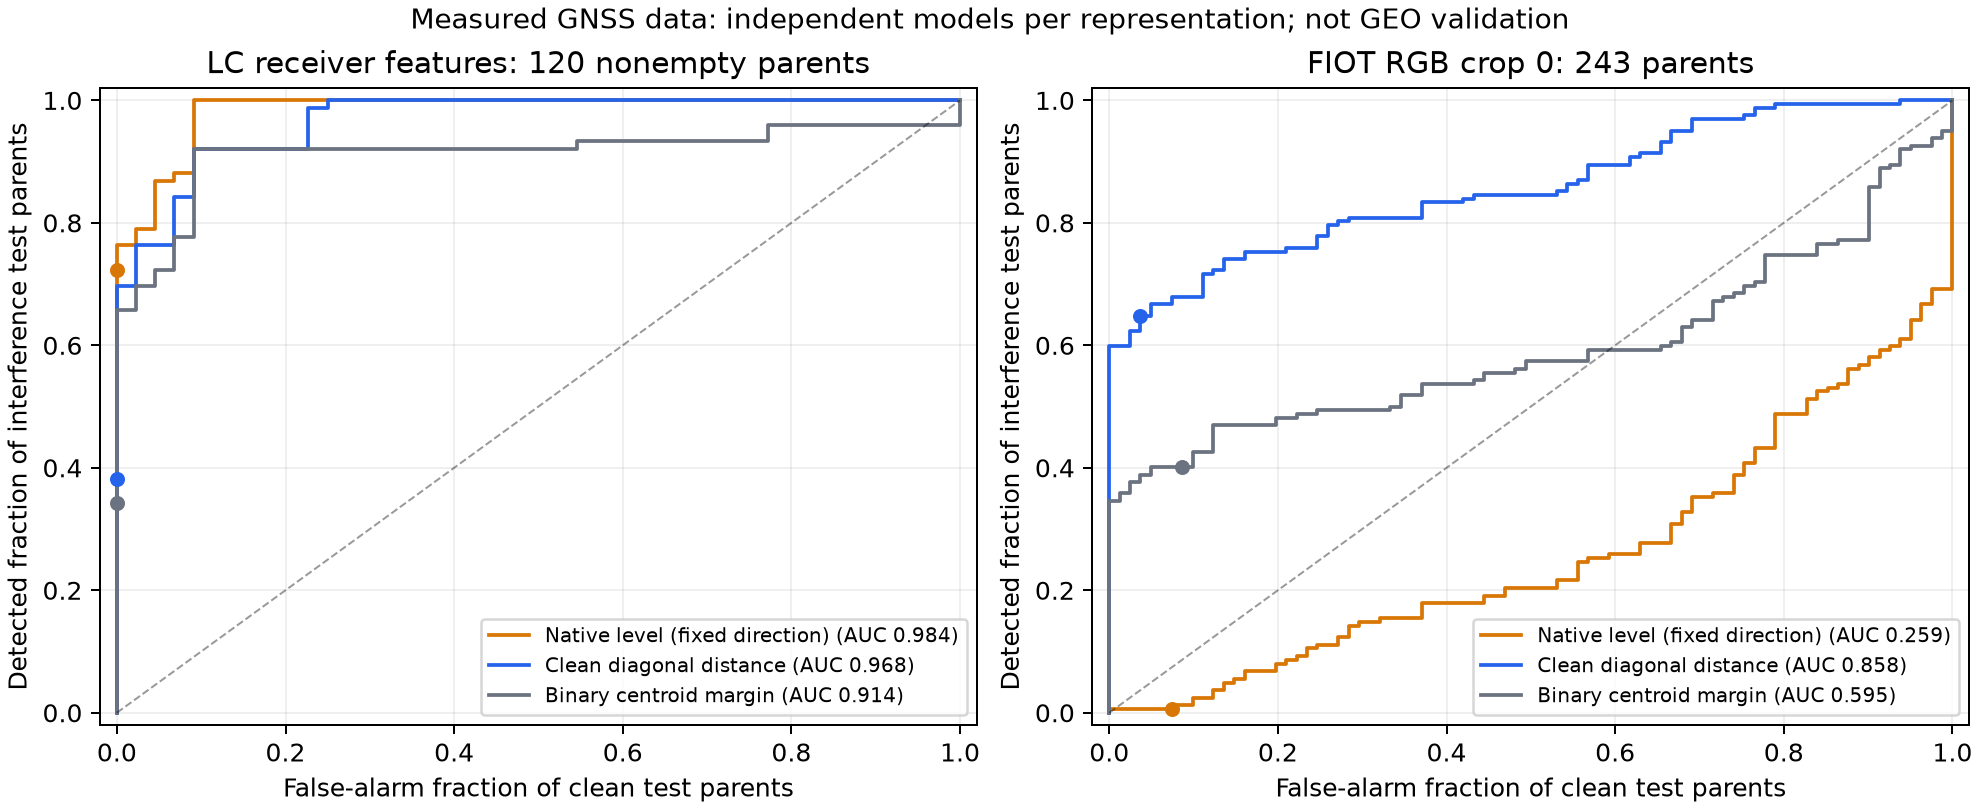
\includegraphics[width=0.95\textwidth,height=\textheight]{figures/public_data_roc.png}
\caption{All three scores on each source. Dots denote the frozen
clean-calibrated thresholds; curves summarize held-out rankings, not
tuned operating points. Models are fitted separately by source.}
\end{figure}

\begin{figure}
\centering
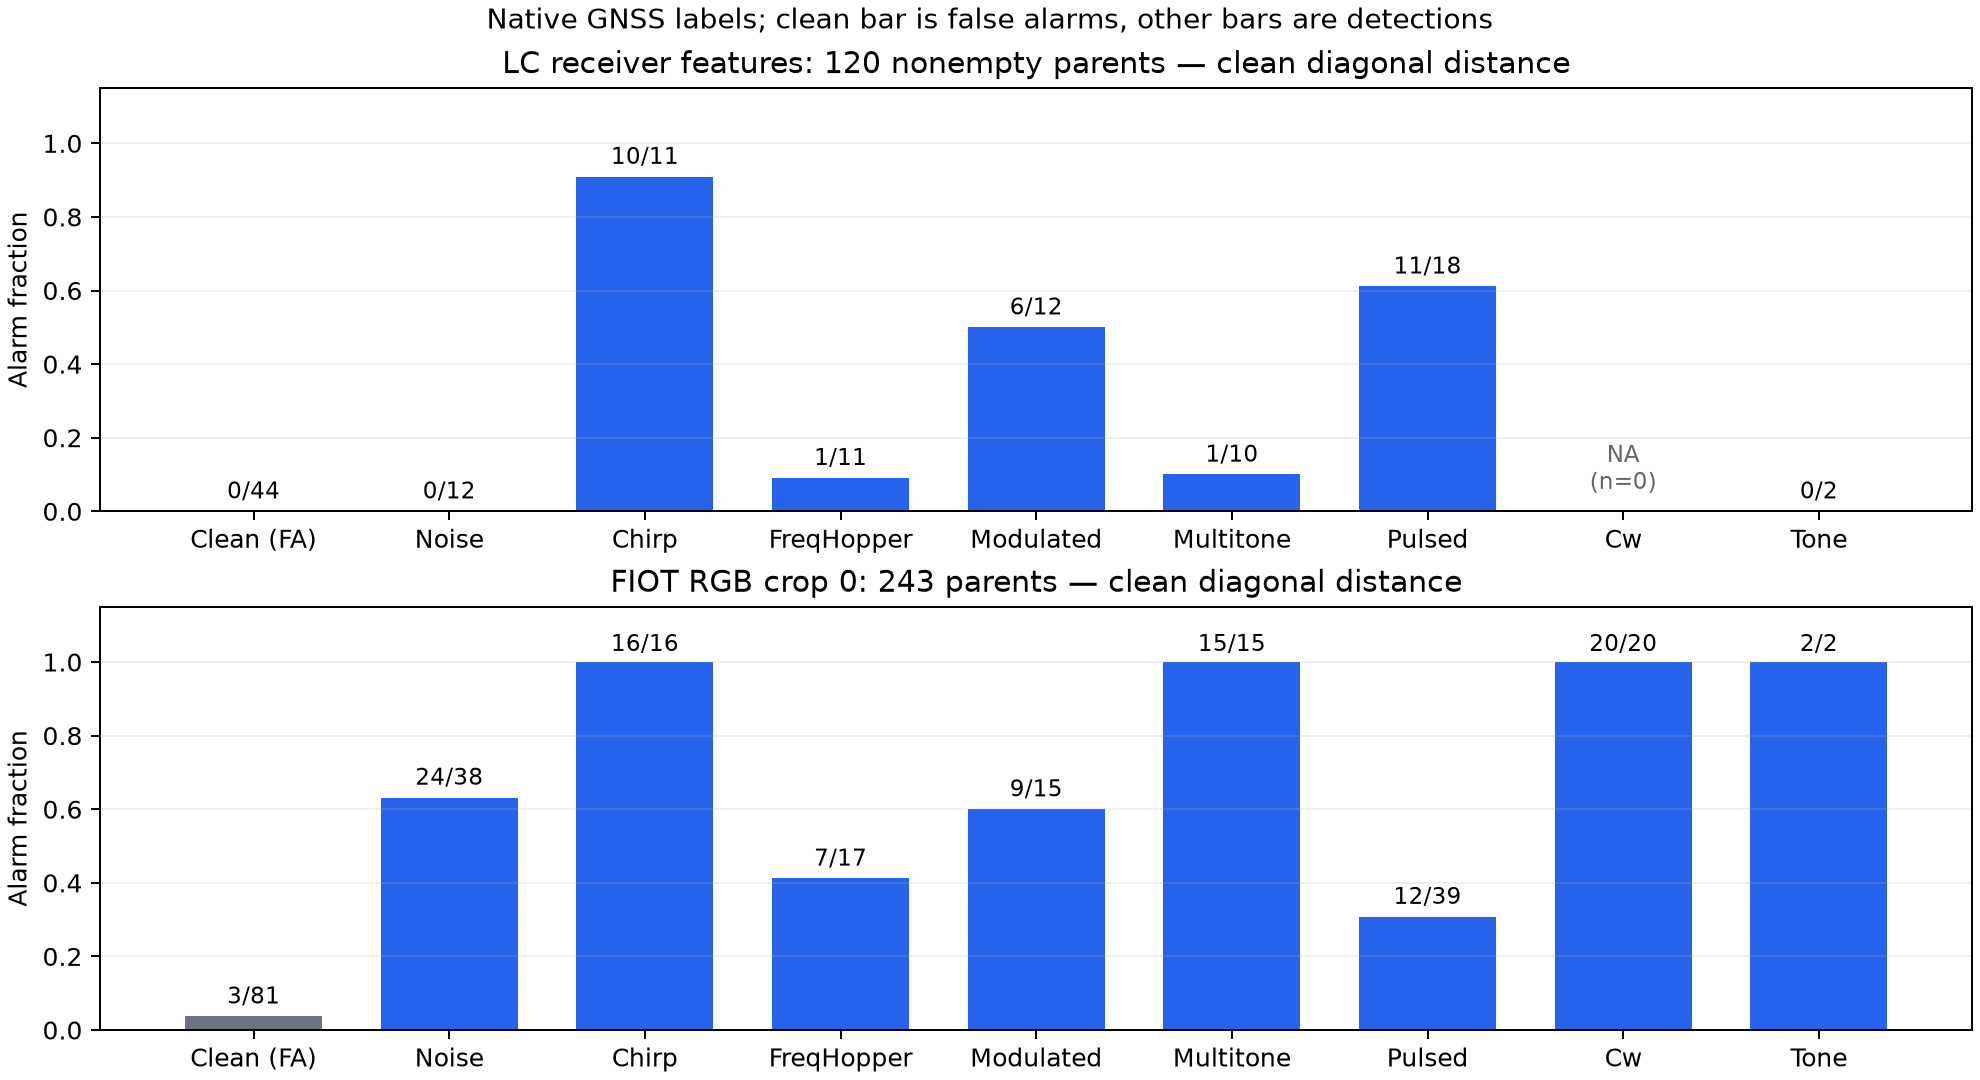
\includegraphics[width=0.95\textwidth,height=\textheight]{figures/public_data_per_class.png}
\caption{Native class counts for the common clean-distance score, an
illustrative stratification rather than a primary scorer selection.
Class 0 is false alarms; LC's absent class 7 is NA. Crop-level repeated
views are not counted as independent recordings.}
\end{figure}

\subsection{Measured amplifier
support}\label{measured-amplifier-support}

\textbf{Table T3. Reused OpenDPD memory-polynomial evidence. NMSE is in
dB; measured outputs are not satellite measurements. Device
technology/frequency attribution follows the preserved project source
audit (P17), rather than a newly verified hardware measurement or a
claim that the current OpenDPD guide documents every device detail.}

\begin{longtable}[]{@{}
  >{\raggedright\arraybackslash}p{(\columnwidth - 8\tabcolsep) * \real{0.1765}}
  >{\raggedright\arraybackslash}p{(\columnwidth - 8\tabcolsep) * \real{0.1765}}
  >{\raggedleft\arraybackslash}p{(\columnwidth - 8\tabcolsep) * \real{0.2353}}
  >{\raggedleft\arraybackslash}p{(\columnwidth - 8\tabcolsep) * \real{0.2353}}
  >{\raggedright\arraybackslash}p{(\columnwidth - 8\tabcolsep) * \real{0.1765}}@{}}
\toprule\noalign{}
\begin{minipage}[b]{\linewidth}\raggedright
Data/device
\end{minipage} & \begin{minipage}[b]{\linewidth}\raggedright
Order / memory setting
\end{minipage} & \begin{minipage}[b]{\linewidth}\raggedleft
Validation NMSE
\end{minipage} & \begin{minipage}[b]{\linewidth}\raggedleft
Test NMSE
\end{minipage} & \begin{minipage}[b]{\linewidth}\raggedright
Support limit
\end{minipage} \\
\midrule\noalign{}
\endhead
\bottomrule\noalign{}
\endlastfoot
APA: GaN Doherty, 3.5 GHz & 5 / 3 & -31.04 & -30.64 & Measured amplitude
envelope; no TWTA saturation validation \\
DPA: CMOS digital Doherty, 2.4 GHz & 5 / 16 & -33.78 & -33.89 & Memory
setting reaches tested grid edge \\
\end{longtable}

The artifact's basis convention uses amplitude powers below the stored
order setting; the label ``order 5'' is the code's setting, not a claim
that the highest exponent is five. These results demonstrate that the
existing artifact reproduces its native test measurements under its
normalization. They do not establish a unique physical nonlinear channel
model, out-of-support amplitude accuracy or GEO hardware generalization.
Bandwidth-rescaled memory and mapping input RMS to nominal IBO 11 dB
remain assumptions. No new PA fit, WebLab measurement or hardware
experiment is included.

\subsection{Simulated GEO observability and physical
consistency}\label{simulated-geo-observability-and-physical-consistency}

\textbf{Table T4. Controlled simulated diagnostics. These rows are
separate populations, not a common detection test.}

\begin{longtable}[]{@{}
  >{\raggedright\arraybackslash}p{(\columnwidth - 6\tabcolsep) * \real{0.2500}}
  >{\raggedright\arraybackslash}p{(\columnwidth - 6\tabcolsep) * \real{0.2500}}
  >{\raggedright\arraybackslash}p{(\columnwidth - 6\tabcolsep) * \real{0.2500}}
  >{\raggedright\arraybackslash}p{(\columnwidth - 6\tabcolsep) * \real{0.2500}}@{}}
\toprule\noalign{}
\begin{minipage}[b]{\linewidth}\raggedright
Diagnostic
\end{minipage} & \begin{minipage}[b]{\linewidth}\raggedright
Population/configuration
\end{minipage} & \begin{minipage}[b]{\linewidth}\raggedright
Existing result
\end{minipage} & \begin{minipage}[b]{\linewidth}\raggedright
Interpretation boundary
\end{minipage} \\
\midrule\noalign{}
\endhead
\bottomrule\noalign{}
\endlastfoot
Reference nonlinear TWTA NPR & One notched-noise seed, amplifier alone &
15.7 to 20.7 dB at IBO 10 to 14 dB; slope about 1.25 dB/dB & No
complete-channel or measured-device validation \\
ASI geometry/visibility & 120 single-pol groups, fixed IBO 11 dB and C/N
25 dB & Median PSD-referenced C/I 20.3 dB; in-plan contrast weak
relative to spill & Antenna/pointing distributions assumed;
event/no-event twin is oracle diagnostic \\
CuC visibility & 24 groups at each of six levels; same fixed-link
setting & Median contrast 0.373 dB at total-plan C/I 20 dB; 0.041 dB at
30 dB & PSD contrast is not operational probability of detection \\
P20 cancellation & 64 scenes, 8 groups, 8 scenes/class across four roles
& Mean active-carrier core-depth range 12.78 to 16.47 dB; paired CuC
median contrast 0.986 to 6.461 dB, 8/8 improve & Diagnostic bands use
truth offline; no learned-model performance claim \\
\end{longtable}

\begin{figure}
\centering
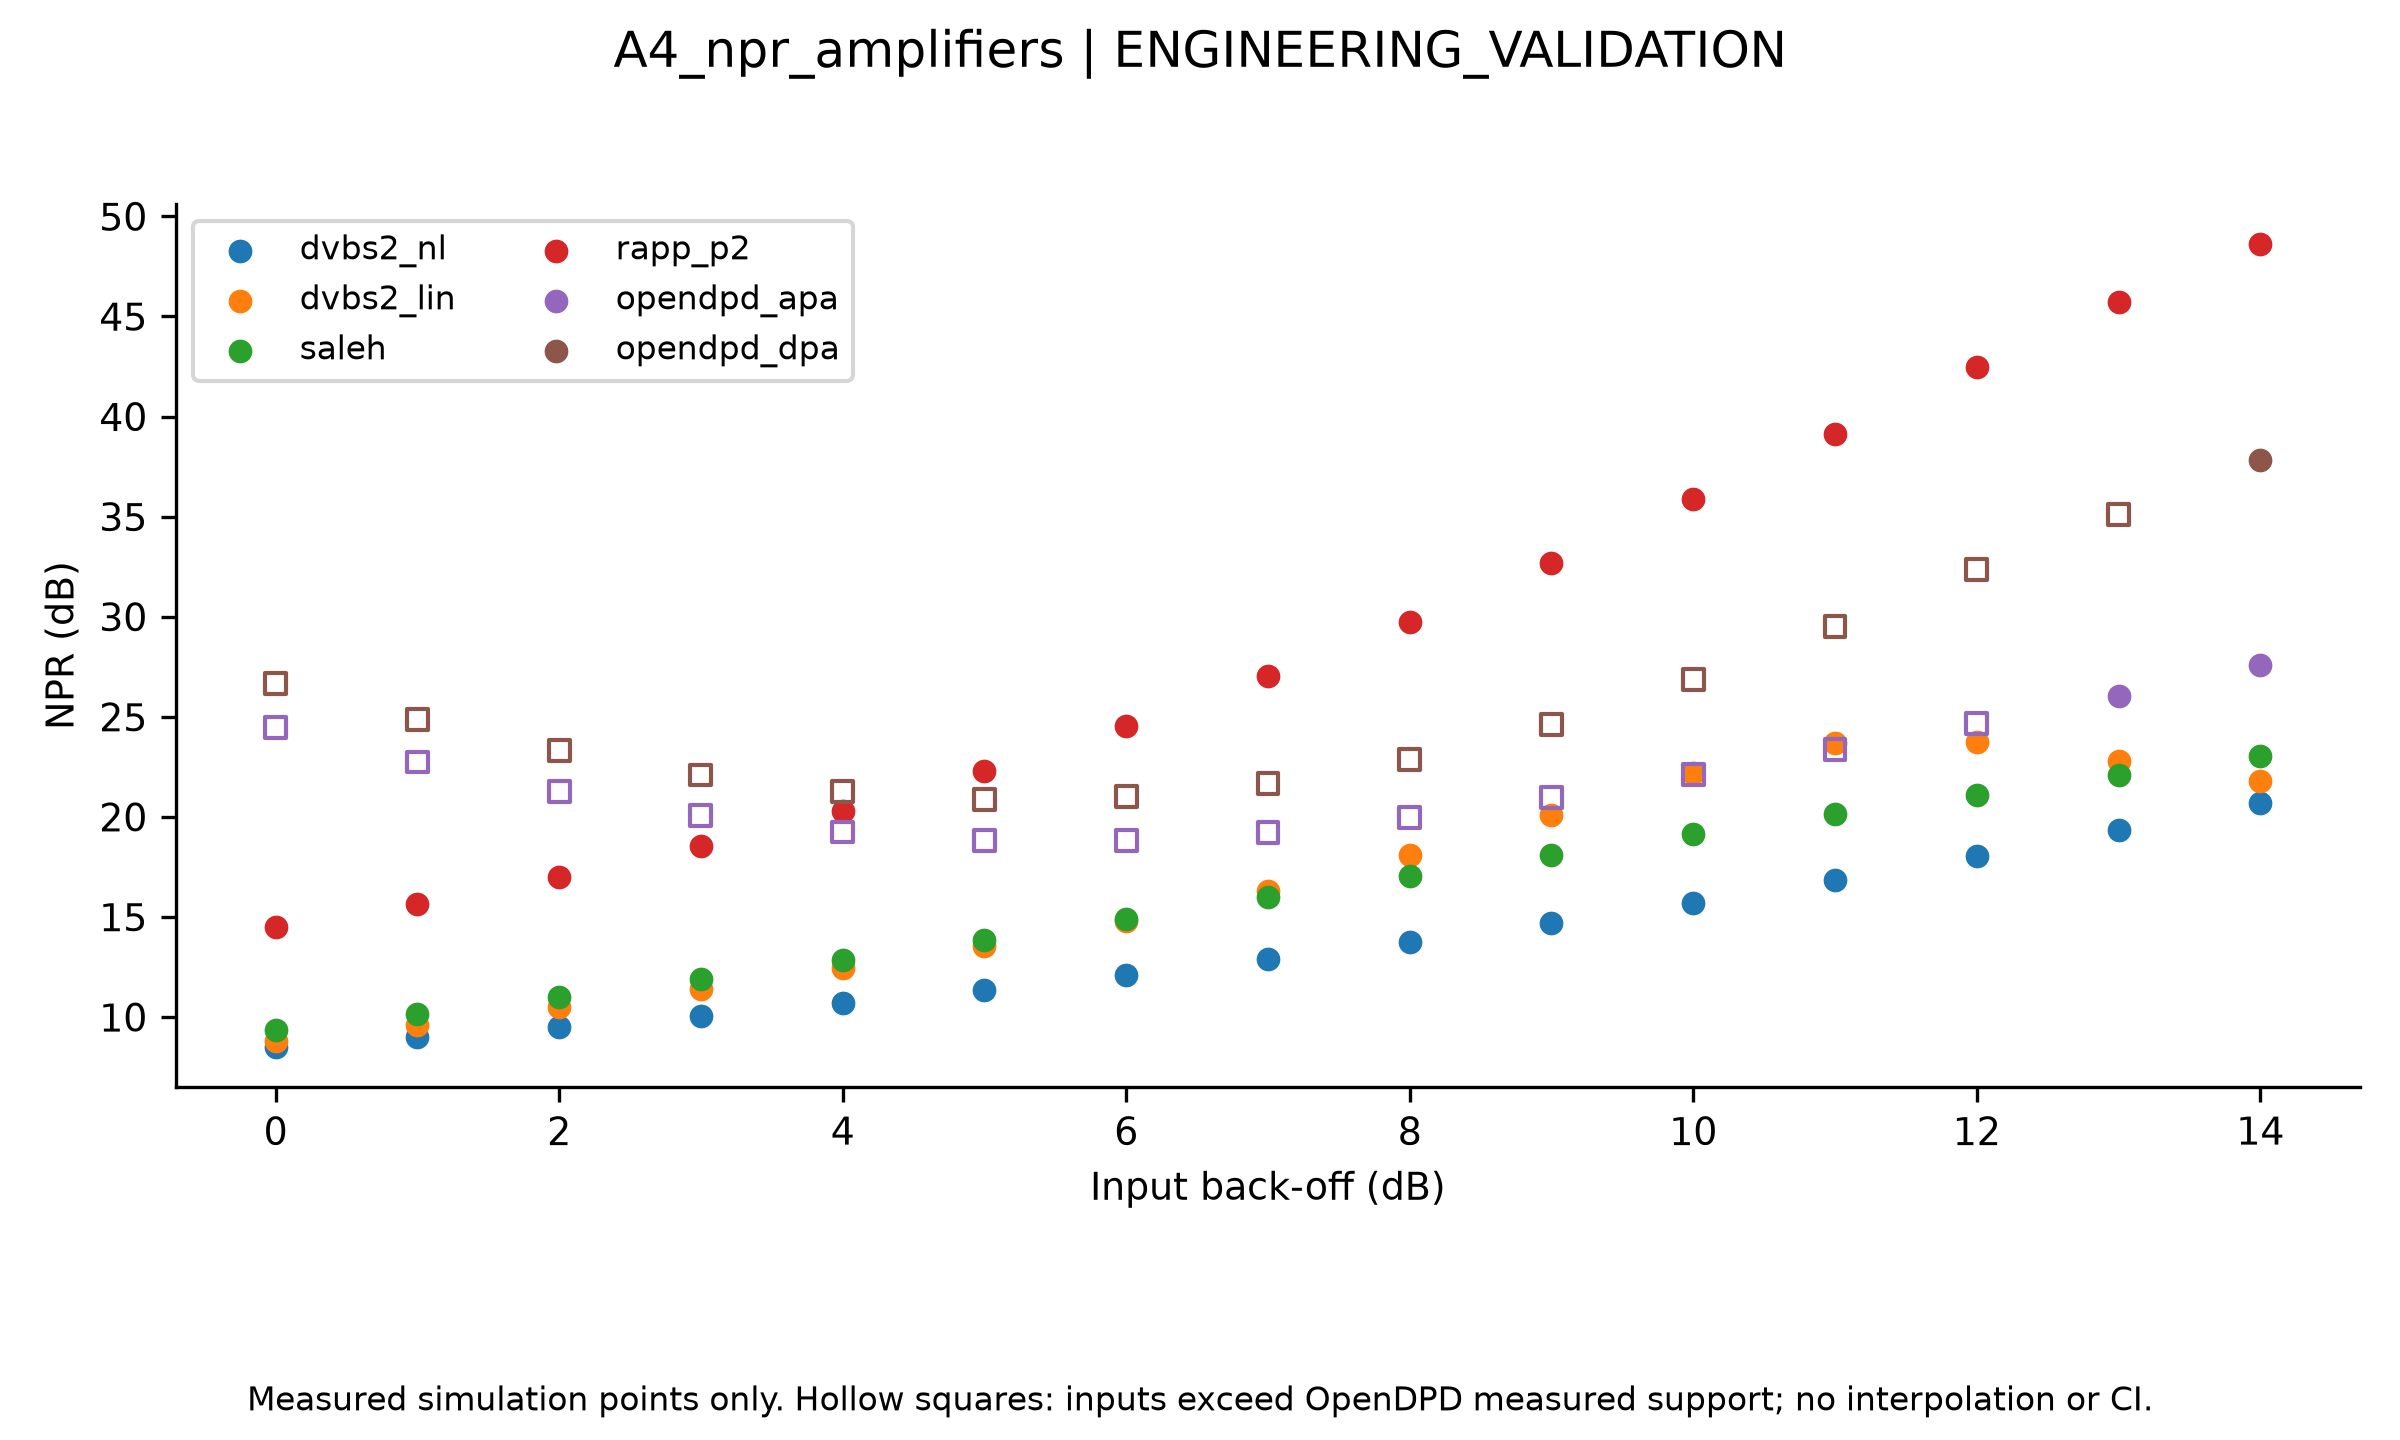
\includegraphics[width=0.95\textwidth,height=\textheight]{figures/npr_amplifiers.png}
\caption{Standalone-amplifier NPR against input back-off. OpenDPD curves
are simulated responses of fitted measured-PA models, not fresh
amplifier measurements; out-of-support inputs are marked in the original
figure.}
\end{figure}

\begin{figure}
\centering
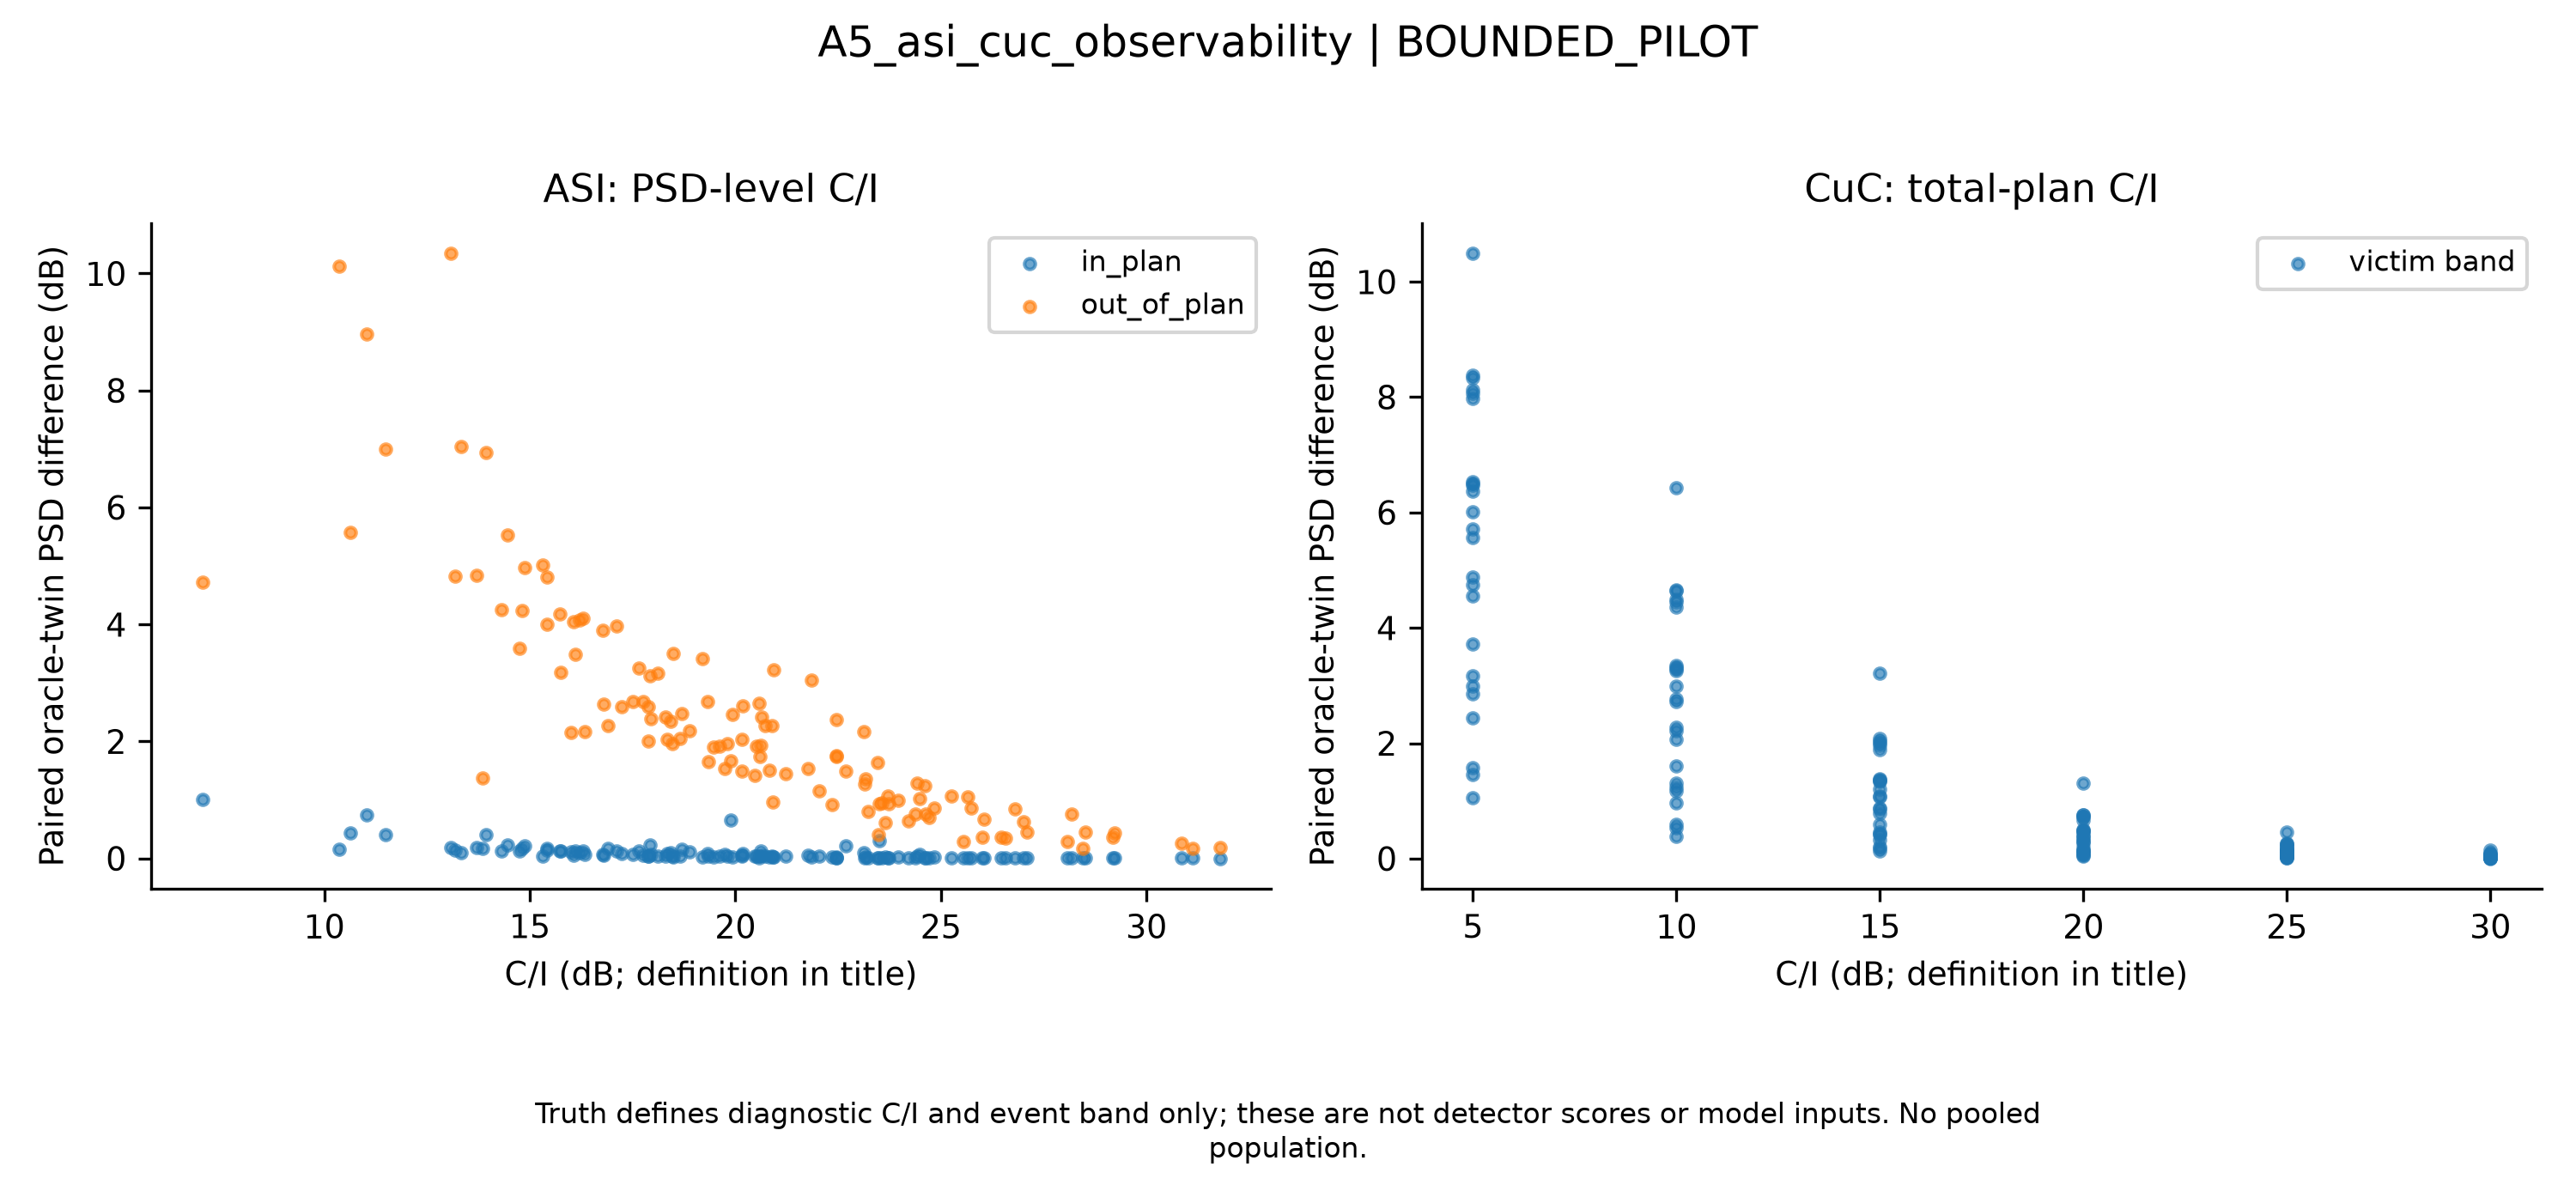
\includegraphics[width=0.95\textwidth,height=\textheight]{figures/asi_cuc_observability.png}
\caption{Separate ASI and CuC controlled visibility summaries.
PSD-referenced and total-plan C/I definitions differ. The observable
contrast uses matched no-event twins and cannot be interpreted as
detector performance.}
\end{figure}

The H.2 linearized-reference NPR curve turns down at low drive; the
existing investigation attributes this to sparse digitized
phase/transfer behavior. It is retained as a model artifact, not
described as a discovered device phenomenon. The NPR and visibility
plots are reused from committed, hash-bound summaries; no figure
regeneration reads RF observations or reruns the simulator.

\section{Physical interpretation and representation
limits}\label{physical-interpretation-and-representation-limits}

The native LC level score associates degraded receiver-reported strength
with the supplied interference labels. That association may exploit
receiver-specific behavior and does not prove a universal
interference-energy mechanism. The FIOT result demonstrates why
replacing such a statistic with a similarly named image statistic is
unsafe: RGB levels depend on the rendering pipeline, and high physical
interference power need not imply a larger stored color mean. A
below-chance score is not evidence that all image features fail; nor
does a stronger distance ranking validate a physical power
interpretation.

The GEO diagnostics explain a different limitation. A weak carrier
underneath a stronger planned carrier can produce little PSD contrast.
Cancellation may expose contrast, but its residual also contains
receiver error and payload distortion. An amplifier-induced product is
not necessarily an external interferer. ASI/unauthorized distinctions
can additionally depend on plan context or geometry, neither of which
exists in the released GNSS inputs. Missing observables cannot be
supplied by relabeling or synthetic metadata appended to the measured
examples.

The measured PA fits support sensitivity to an alternative nonlinear
response only within their native data support and stated mapping
assumptions. A solid-state Doherty response and a TWTA reference curve
differ in device technology and operating region. Their qualitative
comparison is useful for checking an assumption; their juxtaposition is
not evidence that a model transfers to a satellite. Similarly, neither
successful GNSS detection nor a controlled GEO diagnostic establishes
cross-dataset generalization.

\section{Discussion and preserved negative
findings}\label{discussion-and-preserved-negative-findings}

\textbf{Table S1. Historical exploratory findings retained without
conversion to confirmatory results.}

\begin{longtable}[]{@{}
  >{\raggedright\arraybackslash}p{(\columnwidth - 4\tabcolsep) * \real{0.3333}}
  >{\raggedright\arraybackslash}p{(\columnwidth - 4\tabcolsep) * \real{0.3333}}
  >{\raggedright\arraybackslash}p{(\columnwidth - 4\tabcolsep) * \real{0.3333}}@{}}
\toprule\noalign{}
\begin{minipage}[b]{\linewidth}\raggedright
Source
\end{minipage} & \begin{minipage}[b]{\linewidth}\raggedright
Result
\end{minipage} & \begin{minipage}[b]{\linewidth}\raggedright
Why it cannot establish the original full claim
\end{minipage} \\
\midrule\noalign{}
\endhead
\bottomrule\noalign{}
\endlastfoot
A1 Pilot A, two training seeds and about 6\% planned data &
Linear-trained accuracy 78.7\% on linear versus 76.8\% on nonlinear
test; intervals overlap & A statistically confirmed accuracy payload gap
is unsupported \\
R1, one training seed, common four-class models & IBO-shift clean alarms
14/60 for linear-trained versus 1/60 for nonlinear-trained; accuracies
79.1\%/83.7\% & Exploratory fixed-threshold transfer, not multi-seed
confirmation \\
R1 five-class model & Shifted-condition clean alarm rates about
18--27\%; Rapp overdrive 59/60 predicted clean & Labels based on drive
cause need not be identifiable across amplifier families \\
A1 plan intervention, one training seed & A 0.5 MHz plan shift yields
28/30 clean alarms versus 1/30 original & Plan dependence/sensitivity is
not a trained plan-versus-no-plan benefit \\
Canonical P20 tiny neural pilot & 16 training and 16 known-test
observations; 12.5\% known accuracy & Pipeline execution and
observability checks do not establish eight-class recognition \\
\end{longtable}

S1 reports separate historical experiments, not newly computed
estimates. It does not pool their samples or compare a five-class model
against a four-class one as a controlled payload-gap test. The canonical
three-view design contains operator plans in every view; it can test
added polarization/residual observations but cannot by itself identify
learned plan benefit. That would need a separately specified retrained
no-plan control. Unseen carrier-loading generalization also lacks
completed confirmatory evidence.

The practical outcome is a smaller claim than the initial project
ambition. An honest reproducibility paper can document where released
representations and thresholds support conclusions and where they do
not. It must not recast these results as a superior recognizer. A
stronger paper retaining the full C2/C3 claims would require new
predeclared experiments, adequate calibration/test support and separate
execution authorization. Those experiments were not performed for this
manuscript.

\section{Threats to validity}\label{threats-to-validity}

\textbf{Acquisition dependence.} Parent-ID and hash separation do not
rule out shared sessions, receiver settings, jammer hardware or
acquisition schedules. Parent bootstrap may therefore understate
uncertainty. A true session-held-out claim needs additional source
metadata and a separately frozen analysis.

\textbf{Missingness and selection.} LC empties may be nonrandom.
Conditional detection is not population sensitivity; the reported
lower-bound convention is deliberately conservative and still does not
characterize the missing observations. Choosing crop zero reduces
correlation but may discard informative temporal segments. No crop was
selected by detector outcome.

\textbf{Calibration uncertainty.} Clean populations of 38 and 69 records
offer coarse empirical threshold support. A nominal 5\% rule and
matching empirical count do not certify deployment FAR. Fixed-threshold
bootstrap omits recalibration uncertainty and training variability. The
positive centroid also depends on the available mixture of training
interferers.

\textbf{Multiplicity and post hoc interpretation.} All three directions
and feature definitions were frozen before the first metrics. Presenting
their outcomes does not authorize picking a winner for a future test on
the same held-out data. The cross-evidence physical discussion is
explanatory and post hoc; it is not a preregistered causal
identification result.

\textbf{Representation and label validity.} Rendered RGB images may
encode display choices. Receiver telemetry can encode proprietary
processing. Native jammer labels are causes in a GNSS experiment, not
general satellite classes. A PSD-only distinction can be physically
nonidentifiable even with correct labels.

\textbf{Historical source and exposure.} Old pilot results are bound to
their original source/protocol identities; changed source cannot
legitimize historical checkpoint reuse. The B2 scientific register
discloses prior test exposure and prospective exclusion sensitivity
obligations. This paper makes no pristine-B2-test claim and opens no
protected observations. Previously exposed simulator summaries are
descriptive evidence, not a fresh confirmatory held-out test.

\textbf{Reference-model fidelity.} Digitized reference curves, filter
scaling, finite blocks, assumed antenna/pointing distributions,
fixed-link diagnostics and simplified framing bound realism. Measured PA
records do not close the gap to a measured GEO transponder. Known
reference-curve artifacts remain visible.

\textbf{Access, rights and replication.} Inaccessible SmartSpace files
prevent independent numerical comparison. Fraunhofer's license
discrepancy and separately unspecified data rights limit what can be
redistributed. Committed fitted-state summaries and source hashes
improve auditability but do not substitute for lawful raw-data access or
missing acquisition metadata. Human authorship, rights review and venue
suitability remain publication decisions.

\section{Conclusions}\label{conclusions}

This study shows why interference-detection claims must name their
observable, available population and calibration rule. The LC comparison
is conditioned by substantial empty-record coverage; FIOT preserves a
negative RGB-level finding alongside stronger feature-distance ranking.
A ranking result is not a fixed-FAR guarantee, and native GNSS evidence
does not validate GEO deployment. Existing PA fits and controlled
satellite simulations provide complementary, separately scoped evidence
about amplifier support and physical observability.

The completed comparison supports an auditable
reproducibility/comparative-methods contribution. It does not establish
a new recognition algorithm, measured GEO field validity, cross-source
transfer, eight-class open-set superiority or a statistically confirmed
payload gap. The immediate publication work is rights clarification,
author/venue decisions and revision of this complete draft, rather than
another architecture or an unbounded synthetic campaign.

\section{Reproducibility and data
availability}\label{reproducibility-and-data-availability}

The manuscript baseline is repository commit
\texttt{7f58150bbcb674cb9985bcfa4ed56391f3b91c8a}, containing merged PRs
44 and 45. The public-data detector/protocol were fixed at
\texttt{13f79f9ffc824029d91c74299cbfe83131ea4cc6}. The acquisition uses
the pinned Fraunhofer author commit stated above; OpenDPD fitting uses
source commit \texttt{cb4c5ea40632a977f2725575534d3f062fcbb652}. Full
file/figure hashes, machine-readable pointers, numerators, units and
source identities are in \texttt{paper/evidence.json}.
\texttt{paper/audit\_evidence.py} checks committed aggregates without
raw observations, simulation, fitting or network access.

Original public-data runs used Python 3.12.14, NumPy 2.5.4, SciPy 1.18.1
and two numerical threads. LC took 0.740 s wall with peak RSS 26,804
KiB; FIOT took 23.117 s with peak RSS 39,184 KiB. These are historical
single-run measurements, not newly repeated benchmarks. The source
recipe and bounded download/extraction instructions are in
\texttt{research/public\_data/README.md}; no raw dataset is embedded in
the manuscript. Existing scientific figures are copied byte-for-byte
with their provenance retained.

Raw LC/FIOT files must be obtained from the cited owners subject to
clarified terms. OpenDPD's original measurements remain at its source
repository. SmartSpace access requires a functioning authorized share;
its results remain unavailable. Neither scripts that produce data nor
model fitting are required to compile this paper or verify its aggregate
evidence. This manuscript task performs only documentation,
source-metadata verification, aggregate arithmetic and rendering checks.
No full B2 generation, training, GPU probe, LOKO, D-5 sensitivity or
protected held-out evaluation is executed or authorized. Scientific
ratification is not compute permission; the canonical benchmark remains
incomplete.

\section{References}\label{references}

\phantomsection\label{refs}
\begin{CSLReferences}{1}{0}
\bibitem[\citeproctext]{ref-brieger2022multimodal}
Brieger, Tobias, Nisha Lakshmana Raichur, Dorsaf Jdidi, Felix Ott,
Tobias Feigl, J. Rossouw van der Merwe, Alexander Rügamer, and Wolfgang
Felber. 2022. {``Multimodal Learning for Reliable Interference
Classification in {GNSS} Signals.''} In \emph{Proceedings of the 35th
International Technical Meeting of the Satellite Division of the
Institute of Navigation (ION GNSS+ 2022)}, 3210--34.
\url{https://doi.org/10.33012/2022.18586}.

\bibitem[\citeproctext]{ref-fraunhoferLCdataset}
Brieger, Tobias, Nisha Lakshmana Raichur, Dorsaf Jdidi, Felix Ott,
Tobias Feigl, Johannes Rossouw van der Merwe, Alexander Rügamer, and
Wolfgang Felber. 2026. {``Spectrum and Low-Cost ({LC}) Laboratory
Dataset for Interference Classification in {GNSS} Data.''} Zenodo.
\url{https://doi.org/10.5281/zenodo.21333335}.

\bibitem[\citeproctext]{ref-daoud2023dataset}
Daoud, Saed, Geoffrey Eappen, Flor Ortiz, Eva Lagunas, Wallace Martins,
and Symeon Chatzinotas. 2023. {``{CNN}-Based on-Board Interference
Detection in Satellite Systems: An Analysis of Dataset Impact on
Performance.''} In \emph{2023 IEEE International Conference on
Acoustics, Speech, and Signal Processing Workshops (ICASSPW)}, 1--5.
\url{https://doi.org/10.1109/ICASSPW59220.2023.10193395}.

\bibitem[\citeproctext]{ref-etsi2014dvbs2}
ETSI. 2014. {``{EN 302 307-1 V1.4.1}: Digital Video Broadcasting
({DVB}); Second Generation Framing Structure, Channel Coding and
Modulation Systems; Part 1: {DVB-S2}.''}
\url{https://www.etsi.org/deliver/etsi_en/302300_302399/30230701/01.04.01_60/en_30230701v010401p.pdf}.

\bibitem[\citeproctext]{ref-etsi2021dvbs2guide}
---------. 2021. {``{TR 102 376-2 V1.2.1}: Digital Video Broadcasting
({DVB}); Implementation Guidelines for the Second Generation System;
Part 2: {S2} Extensions ({DVB-S2X}).''}
\url{https://www.etsi.org/deliver/etsi_tr/102300_102399/10237602/01.02.01_60/tr_10237602v010201p.pdf}.

\bibitem[\citeproctext]{ref-henarejos2019interference}
Henarejos, Pol, Miguel Ángel Vázquez, and Ana Isabel Pérez-Neira. 2019.
{``Deep Learning for Experimental Hybrid Terrestrial and Satellite
Interference Management.''} \url{https://arxiv.org/abs/1906.03012}.

\bibitem[\citeproctext]{ref-heublein2024robustness}
Heublein, Lucas, Tobias Feigl, Thorsten Nowak, Alexander Rügamer,
Christopher Mutschler, and Felix Ott. 2025. {``Evaluating {ML}
Robustness in {GNSS} Interference Classification, Characterization \&
Localization.''} In \emph{2025 International Conference on Localization
and GNSS (ICL-GNSS)}, 1--7.
\url{https://doi.org/10.1109/ICL-GNSS65520.2025.11046126}.

\bibitem[\citeproctext]{ref-heublein2024discrepancies}
Heublein, Lucas, Nisha L. Raichur, Tobias Feigl, Tobias Brieger, Fin
Heuer, Lennart Asbach, Alexander Rügamer, and Felix Ott. 2024.
{``Evaluation of (Un-)supervised Machine Learning Methods for {GNSS}
Interference Classification with Real-World Data Discrepancies.''} In
\emph{Proceedings of the 37th International Technical Meeting of the
Satellite Division of the Institute of Navigation (ION GNSS+ 2024)},
1260--93. \url{https://doi.org/10.33012/2024.19887}.

\bibitem[\citeproctext]{ref-pellaco2019spectrum}
Pellaco, Lissy, Nirankar Singh, and Joakim Jaldén. 2019. {``Spectrum
Prediction and Interference Detection for Satellite Communications.''}
\url{https://arxiv.org/abs/1912.04716}.

\bibitem[\citeproctext]{ref-politis2017weak}
Politis, Christos, Sina Maleki, Christos Tsinos, Symeon Chatzinotas, and
Björn Ottersten. 2017. {``Weak Interference Detection with Signal
Cancellation in Satellite Communications.''} In \emph{2017 IEEE
International Conference on Acoustics, Speech and Signal Processing
(ICASSP)}, 6289--93. \url{https://doi.org/10.1109/ICASSP.2017.7953366}.

\bibitem[\citeproctext]{ref-saifaldawla2024genai}
Saifaldawla, Almoatssimbillah, Flor Ortiz, Eva Lagunas, Abuzar B. M.
Adam, and Symeon Chatzinotas. 2024. {``{GenAI}-Based Models for {NGSO}
Satellites Interference Detection.''} \emph{IEEE Transactions on Machine
Learning in Communications and Networking} 2: 904--24.
\url{https://doi.org/10.1109/TMLCN.2024.3418933}.

\bibitem[\citeproctext]{ref-saleh1981twta}
Saleh, Adel A. M. 1981. {``Frequency-Independent and Frequency-Dependent
Nonlinear Models of {TWT} Amplifiers.''} \emph{IEEE Transactions on
Communications} 29 (11): 1715--20.
\url{https://doi.org/10.1109/TCOM.1981.1094911}.

\bibitem[\citeproctext]{ref-smartspaceDatasets}
University of Luxembourg SmartSpace. n.d. {``{SmartSpace} Research
Datasets and Usage Conditions.''} Accessed October 26, 2026.
\url{https://fnr-smartspace-project.uni.lu/datasets/}.

\bibitem[\citeproctext]{ref-wu2024opendpd}
Wu, Yizhuo, Gagan Deep Singh, Mohammadreza Beikmirza, Leo C. N. de
Vreede, Morteza Alavi, and Chang Gao. 2024. {``{OpenDPD}: An Open-Source
End-to-End Learning \& Benchmarking Framework for Wideband Power
Amplifier Modeling and Digital Pre-Distortion.''} In \emph{2024 IEEE
International Symposium on Circuits and Systems (ISCAS)}, 1--5.
\url{https://doi.org/10.1109/ISCAS58744.2024.10558162}.

\end{CSLReferences}

\end{document}
